\section{Design}
% Metatext

\subsection{System design}


\subsection{User Interface Design}
% General Introduction to UI - what + why
The user interface (UI) provides interaction methods between the user and the app.
As the priority of this project is functionality with regards to data collection and route generation and comparison, the UI will not be developed together with users, nor allocated excessive resources. 
The UI is developed for practical purposes, like testing, and to lay the basis for further development, but is still held to some standard which will be documented in the following text. 

\subsubsection{Design language}
% Definition
The design language is the general look and appearance of a system.
This is the foundation for the impressions and feels of the user, and affects the user experience.
The design language is selected in collaboration with another aSTEP project group, SW604f16.

% Goals
The user interface is designed to achieve the following usability characteristics \cite{DIS2014}:
\begin{itemize}
	\item Learnability
	\item Utility
	\item Safety
	\item Effectiveness
\end{itemize}

% Paragraph regarding selection of material
Adhering the material design guidelines makes the app achieve a similar aesthetic and usage method as other apps in the Android eco-system. 
The design is clean and simple, regarding colors and input methods.\todo{maybe clean and simple is bad words?}

% Material design
The UI is designed to mostly comply with the Google's Material design guidelines \cite{materialDesign}, being ``\textit{bold, graphic, intentional}''. 
Some of the Material design properties are stated in the following list, compiled of citations from the design guidelines \cite{materialProperties}:

\begin{enumerate}
	\item Material has varying x \& y dimensions (measured in dp) and a uniform thickness (1dp).
	\item Material casts shadows. Shadows result naturally from the relative elevation (z-position) between material elements.
	\item Content is displayed on material, in any shape and color. Content does not add thickness to material.
	\item Input events cannot pass through material.
	\item Material cannot pass through other material. For example, one sheet of material cannot pass through another sheet of material when changing elevation.
	\item Material grows and shrinks only along its plane.
	\item Material never bends or folds.
	\item Material can be spontaneously generated or destroyed anywhere in the environment.
\end{enumerate} 


\subsubsection{User interface}
% Actions in UI and design thereof
The design drafts in Figure \ref{fig:GUI-firstrun} reflect the necessary functions and the previously described design language. 

% Login and registering pages design
As the user needs a user profile in the aSTEP system to use the app, the users must be able to login if they already have a user profile, or create a new user profile.
\todo{maybe fix figures. UrMomIsNice and loginPic}

\begin{figure}[h!]
	 \centering
	 \begin{subfigure}[b]{0.3\textwidth}
	 	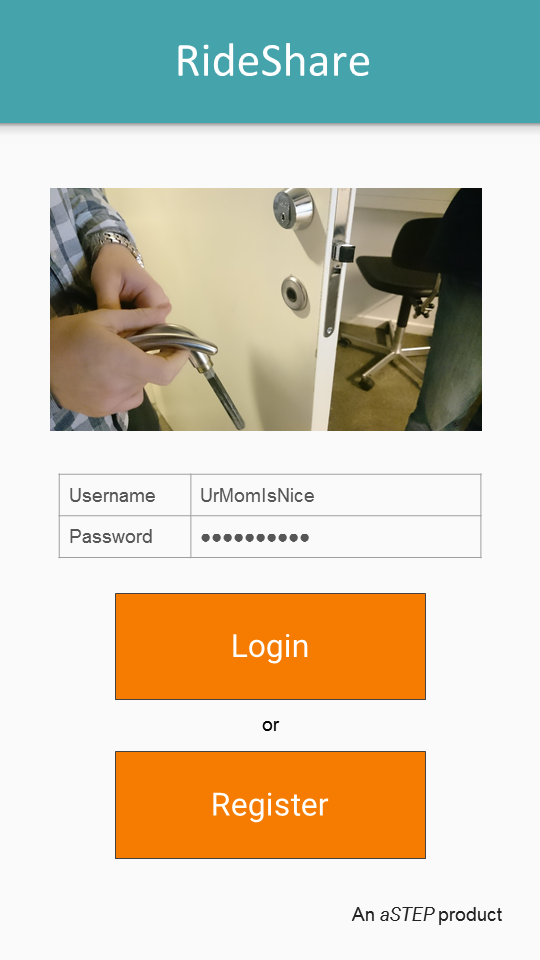
\includegraphics[width=\textwidth]{figures/GUI-front.png}
	 	\caption{Login page}
	 	\label{fig:GUI-front}
	 \end{subfigure}
	 ~ %add desired spacing between images, e. g. ~, \quad, \qquad, \hfill etc. 
	 %(or a blank line to force the subfigure onto a new line)
	 \begin{subfigure}[b]{0.3\textwidth}
	 	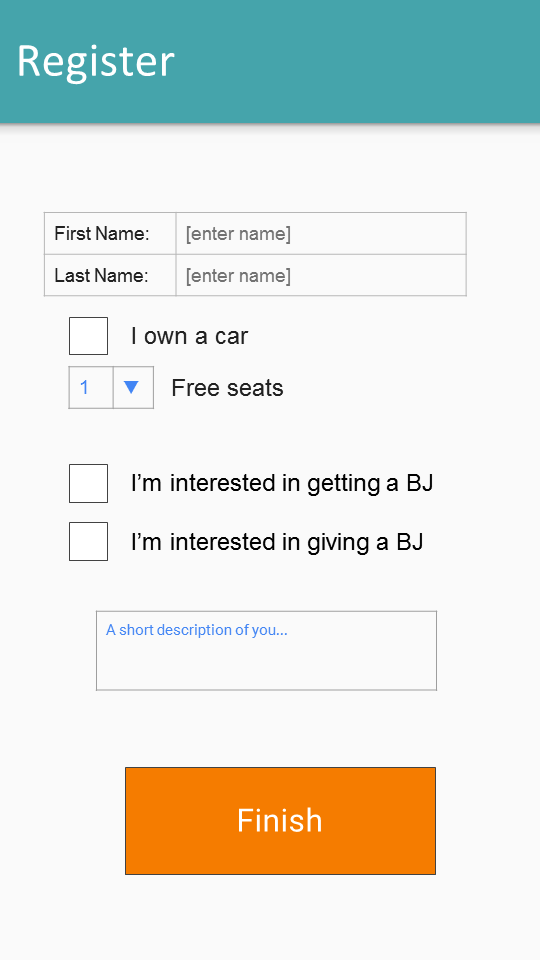
\includegraphics[width=\textwidth]{figures/GUI-register.png}
	 	\caption{Register page}
	 	\label{fig:GUI-register}
	 \end{subfigure}
	 \caption{Draft of the login and registering pages of the app.}\label{fig:GUI-firstrun}
\end{figure}

% In-app pages design
Several screens are necessary to support the different parts of the app. 
The app needs a screen for login, registering, presentation of matches, and a settings page, as can be seen in the figures in Figure \ref{fig:GUI-in-app}.

\begin{figure}[h!]
	\centering
	\begin{subfigure}[b]{0.3\textwidth}
		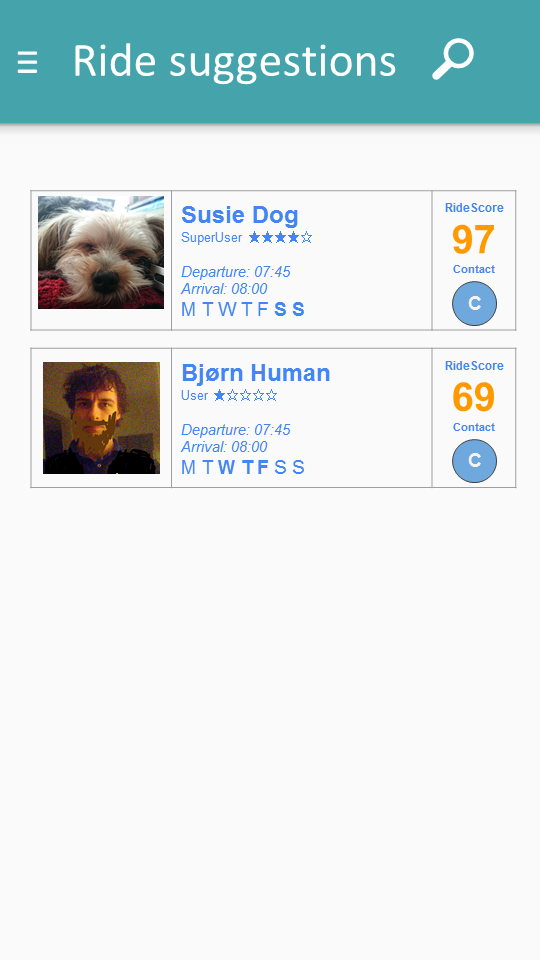
\includegraphics[width=\textwidth]{figures/GUI-main.png}
		\caption{Main page}
		\label{fig:GUI-main}
	\end{subfigure}
	~ %add desired spacing between images, e. g. ~, \quad, \qquad, \hfill etc. 
	%(or a blank line to force the subfigure onto a new line)
	\begin{subfigure}[b]{0.3\textwidth}
		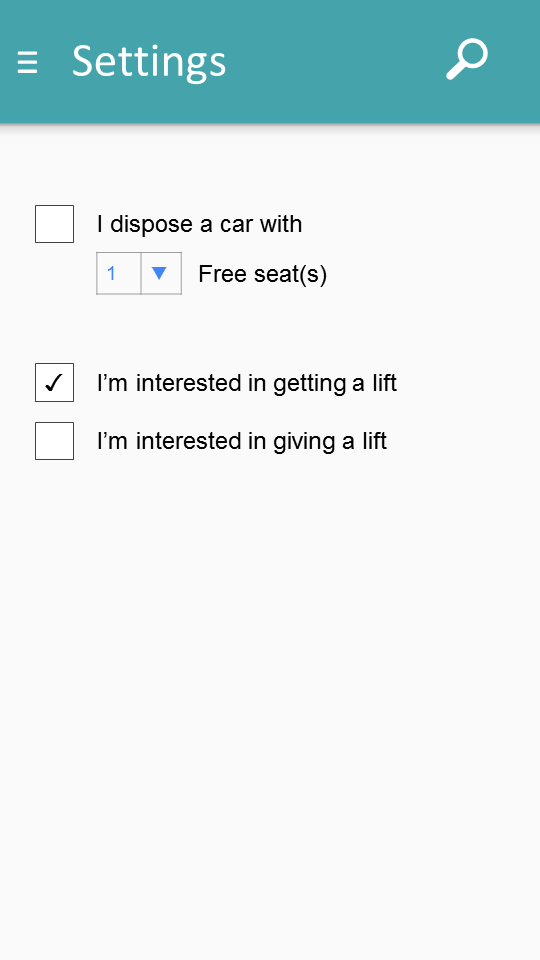
\includegraphics[width=\textwidth]{figures/GUI-settings.png}
		\caption{Settings page}
		\label{fig:GUI-settings}
	\end{subfigure}
	\caption{Draft of the in-app pages of the app.}\label{fig:GUI-in-app}
\end{figure}


